% Options for packages loaded elsewhere
\PassOptionsToPackage{unicode}{hyperref}
\PassOptionsToPackage{hyphens}{url}
%
\documentclass[
]{article}
\usepackage{amsmath,amssymb}
\usepackage{lmodern}
\usepackage{ifxetex,ifluatex}
\ifnum 0\ifxetex 1\fi\ifluatex 1\fi=0 % if pdftex
  \usepackage[T1]{fontenc}
  \usepackage[utf8]{inputenc}
  \usepackage{textcomp} % provide euro and other symbols
\else % if luatex or xetex
  \usepackage{unicode-math}
  \defaultfontfeatures{Scale=MatchLowercase}
  \defaultfontfeatures[\rmfamily]{Ligatures=TeX,Scale=1}
\fi
% Use upquote if available, for straight quotes in verbatim environments
\IfFileExists{upquote.sty}{\usepackage{upquote}}{}
\IfFileExists{microtype.sty}{% use microtype if available
  \usepackage[]{microtype}
  \UseMicrotypeSet[protrusion]{basicmath} % disable protrusion for tt fonts
}{}
\makeatletter
\@ifundefined{KOMAClassName}{% if non-KOMA class
  \IfFileExists{parskip.sty}{%
    \usepackage{parskip}
  }{% else
    \setlength{\parindent}{0pt}
    \setlength{\parskip}{6pt plus 2pt minus 1pt}}
}{% if KOMA class
  \KOMAoptions{parskip=half}}
\makeatother
\usepackage{xcolor}
\IfFileExists{xurl.sty}{\usepackage{xurl}}{} % add URL line breaks if available
\IfFileExists{bookmark.sty}{\usepackage{bookmark}}{\usepackage{hyperref}}
\hypersetup{
  pdftitle={Survey Simulation Example},
  pdfauthor={Eura Nama},
  hidelinks,
  pdfcreator={LaTeX via pandoc}}
\urlstyle{same} % disable monospaced font for URLs
\usepackage[margin=1in]{geometry}
\usepackage{longtable,booktabs,array}
\usepackage{calc} % for calculating minipage widths
% Correct order of tables after \paragraph or \subparagraph
\usepackage{etoolbox}
\makeatletter
\patchcmd\longtable{\par}{\if@noskipsec\mbox{}\fi\par}{}{}
\makeatother
% Allow footnotes in longtable head/foot
\IfFileExists{footnotehyper.sty}{\usepackage{footnotehyper}}{\usepackage{footnote}}
\makesavenoteenv{longtable}
\usepackage{graphicx}
\makeatletter
\def\maxwidth{\ifdim\Gin@nat@width>\linewidth\linewidth\else\Gin@nat@width\fi}
\def\maxheight{\ifdim\Gin@nat@height>\textheight\textheight\else\Gin@nat@height\fi}
\makeatother
% Scale images if necessary, so that they will not overflow the page
% margins by default, and it is still possible to overwrite the defaults
% using explicit options in \includegraphics[width, height, ...]{}
\setkeys{Gin}{width=\maxwidth,height=\maxheight,keepaspectratio}
% Set default figure placement to htbp
\makeatletter
\def\fps@figure{htbp}
\makeatother
\setlength{\emergencystretch}{3em} % prevent overfull lines
\providecommand{\tightlist}{%
  \setlength{\itemsep}{0pt}\setlength{\parskip}{0pt}}
\setcounter{secnumdepth}{-\maxdimen} % remove section numbering
\usepackage{tikz} \usepackage{pdflscape} \usepackage{float}
\newcommand{\blandscape}{\begin{landscape}}
\newcommand{\elandscape}{\end{landscape}}
\ifluatex
  \usepackage{selnolig}  % disable illegal ligatures
\fi

\title{Survey Simulation Example}
\author{Eura Nama}
\date{}

\begin{document}
\maketitle

\hypertarget{survey-parameters}{%
\section{Survey Parameters}\label{survey-parameters}}

Just so you can keep track in the document, we return the survey parameters that you set for this simulation.

\begin{table}

\caption{\label{tab:paras}A Table of your input values for the current run of your simulation}
\centering
\begin{tabular}[t]{ll}
\toprule
Parameter & Value\\
\midrule
Number of Tows & 20\\
Total Biomass & 100000 tonnes\\
Catchability & 0.3\\
Area swept by a tow & 10000 m²\\
Number of Simulations & 4\\
\addlinespace
Biomass distribution & NAFO\\
\bottomrule
\end{tabular}
\end{table}

\hypertarget{survey-simulation}{%
\subsection{Survey Simulation}\label{survey-simulation}}

So now we can review the input data we have for our survey. First we will look at some figures. First off, lets take a look at our survey area, included in this figure are the North Atlantic Fishery Organization (NAFO) subareas that are the basis for the NAFO stratification, and the bathymetry of the region, which is used as the basis of the depth stratification (Figure \ref{fig:base-plt}).

\begin{figure}
\centering
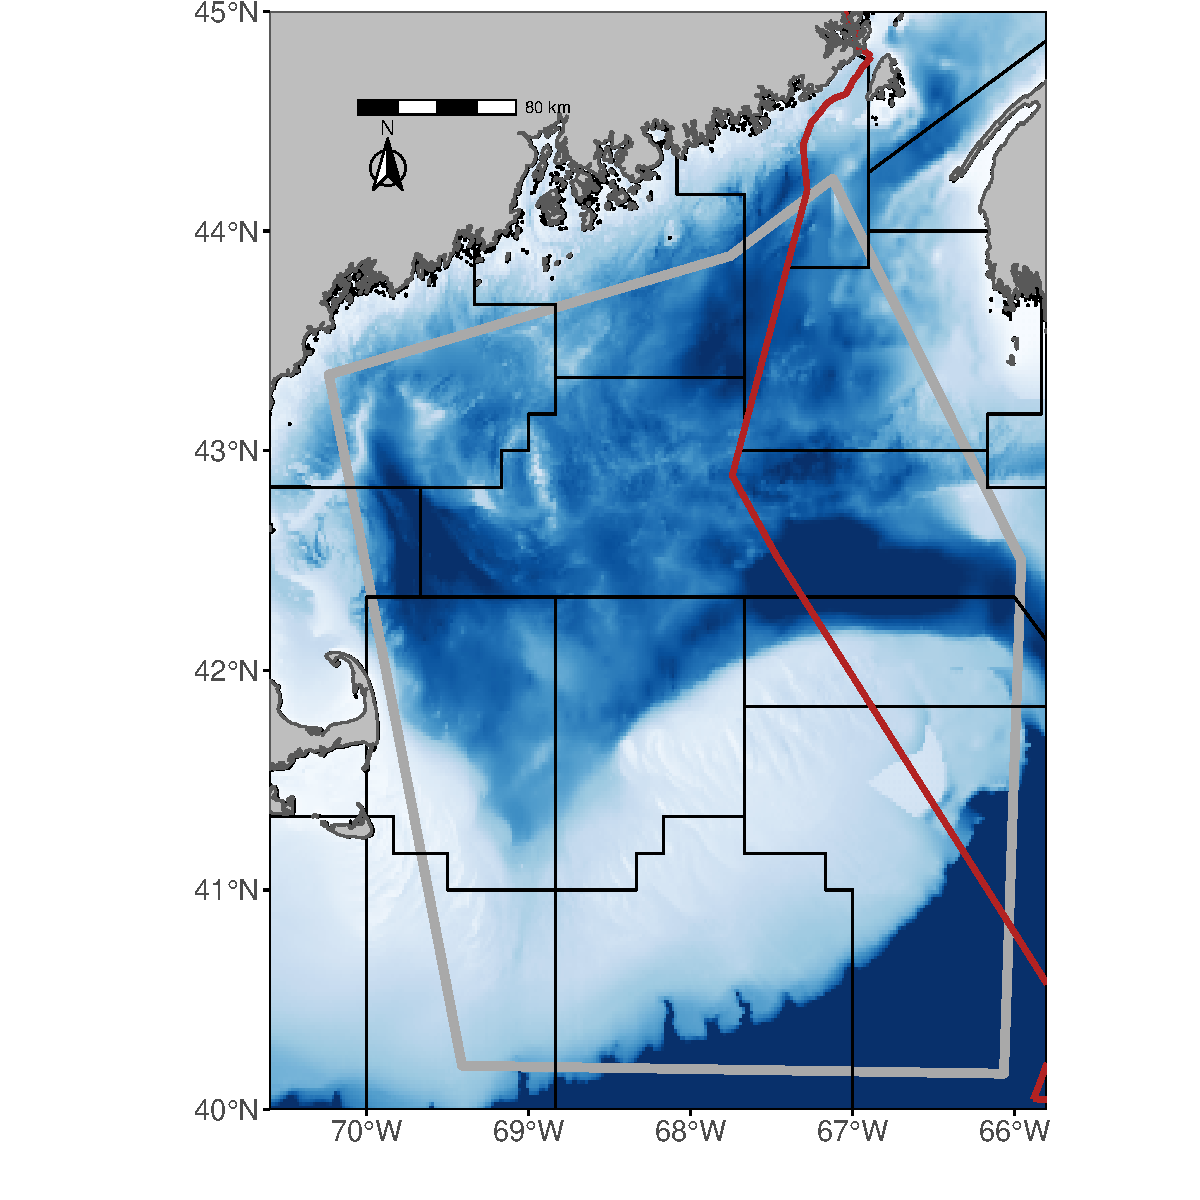
\includegraphics{Survey_tutortial_files/figure-latex/base-plt-1.pdf}
\caption{\label{fig:base-plt}The assessment area for the Dusky Scalloped Shark (\emph{Dustious maximus}) is outlined by the thick grey line. The thin black lines are the NAFO subareas in the region. The red line divides shows the division between the economic exclusive zone (EEZs) for Canada and the United States. The bathymetry in the region is also shown.}
\end{figure}

Now we can also show the distribution of the biomass in the area. If 4 is greater than 1 then we'll show two or three realizations from the models depending on how many simulations we ran. First we show the biomass distribution with the random survey stations overlain (Figure \ref{fig:rand-samp-plt}).

\begin{figure}
\centering
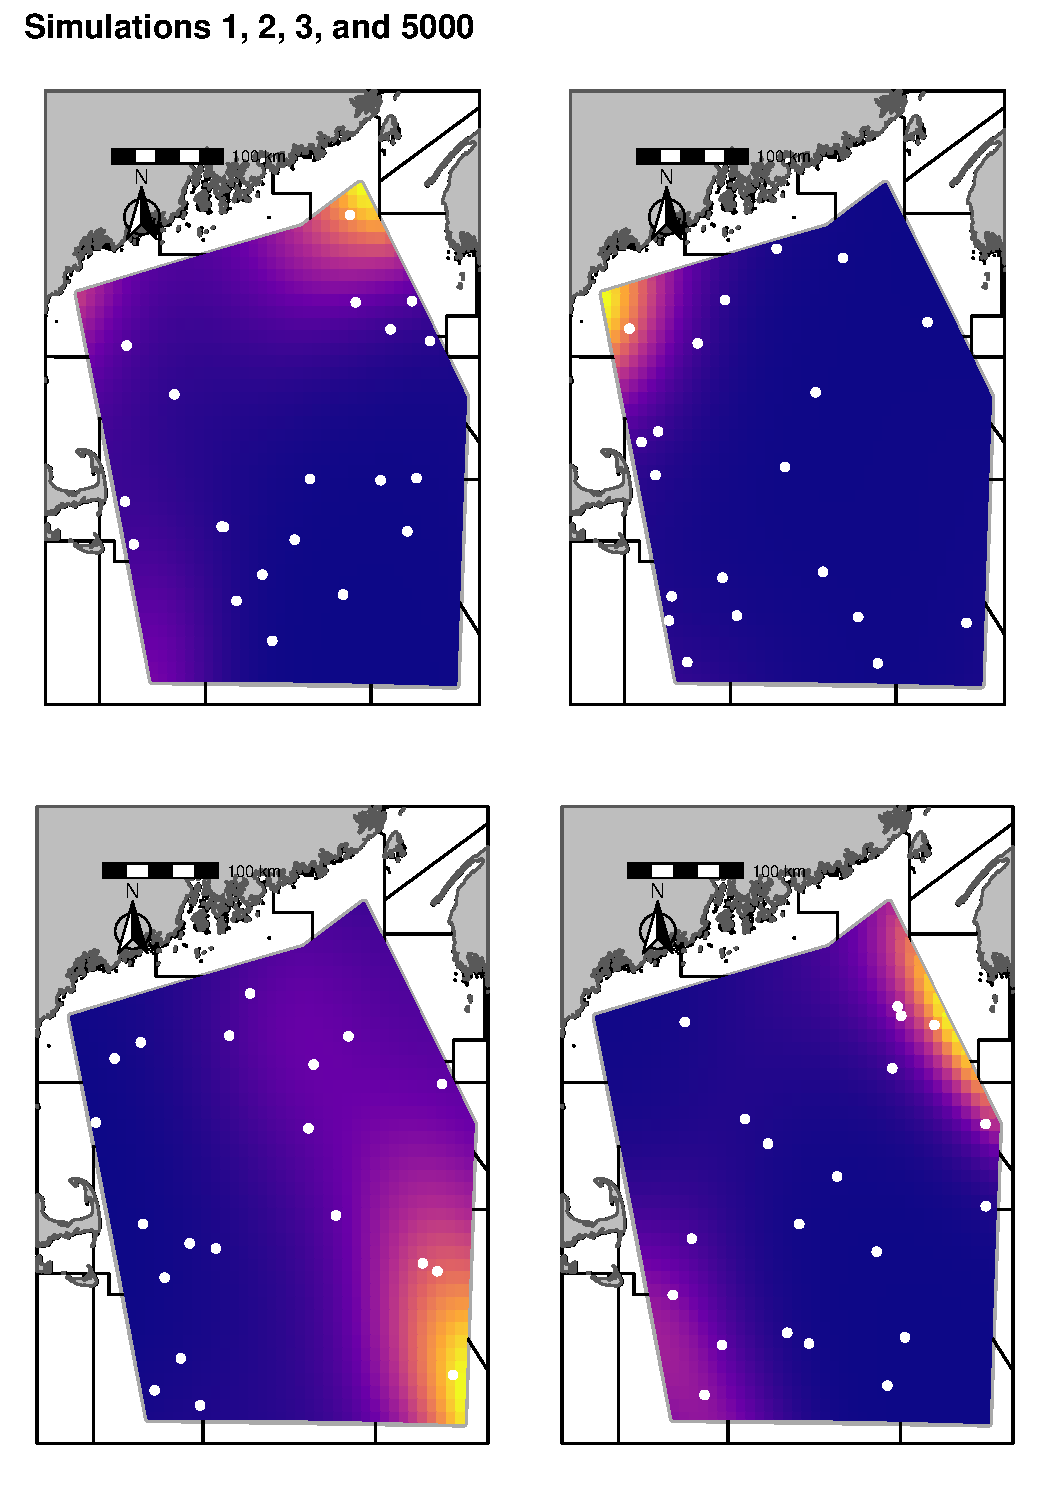
\includegraphics{Survey_tutortial_files/figure-latex/rand-samp-plt-1.pdf}
\caption{\label{fig:rand-samp-plt}Biomass distribution with the random survey stations overlain}
\end{figure}

Next we show the biomass distribution with the NAFO survey stations and NAFO strata overlain (Figure \ref{fig:rand-samp-plt}).

\begin{figure}
\centering
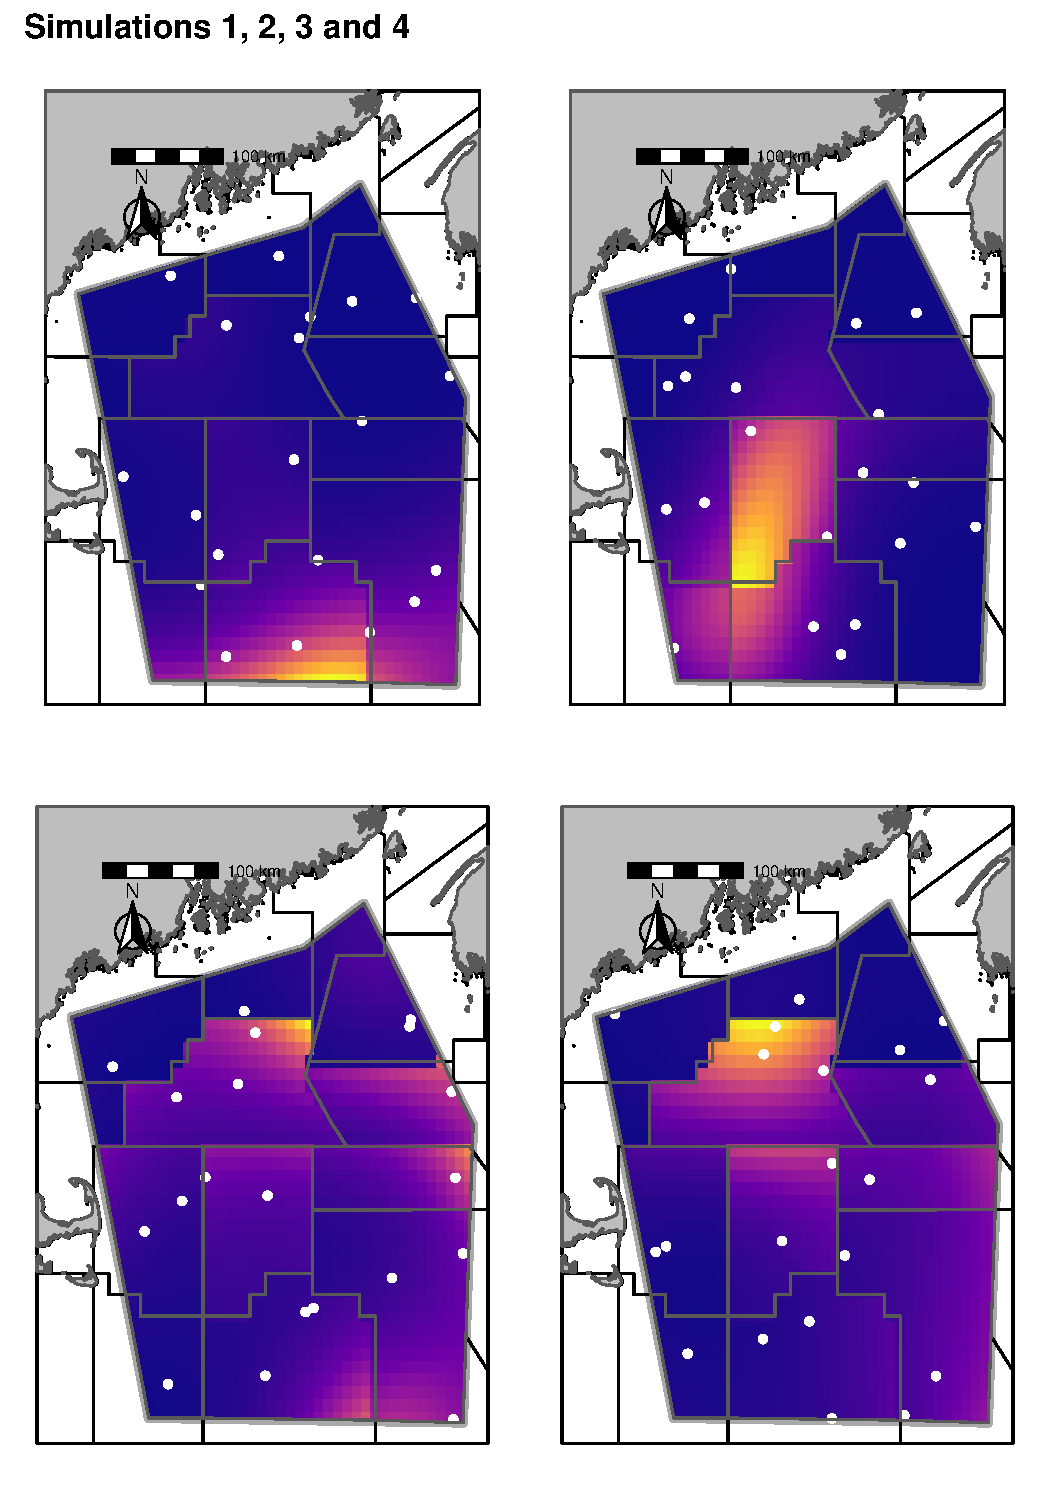
\includegraphics{Survey_tutortial_files/figure-latex/nafo-samp-plt-1.pdf}
\caption{\label{fig:nafo-samp-plt}Biomass distribution with the NAFO survey stations and NAFO stratification polygons overlain}
\end{figure}

Finally, we show the biomass distribuiton with the Depth survey stations and Depth stratification overlain (Figure \ref{fig:depth-samp-plt})

\begin{figure}
\centering
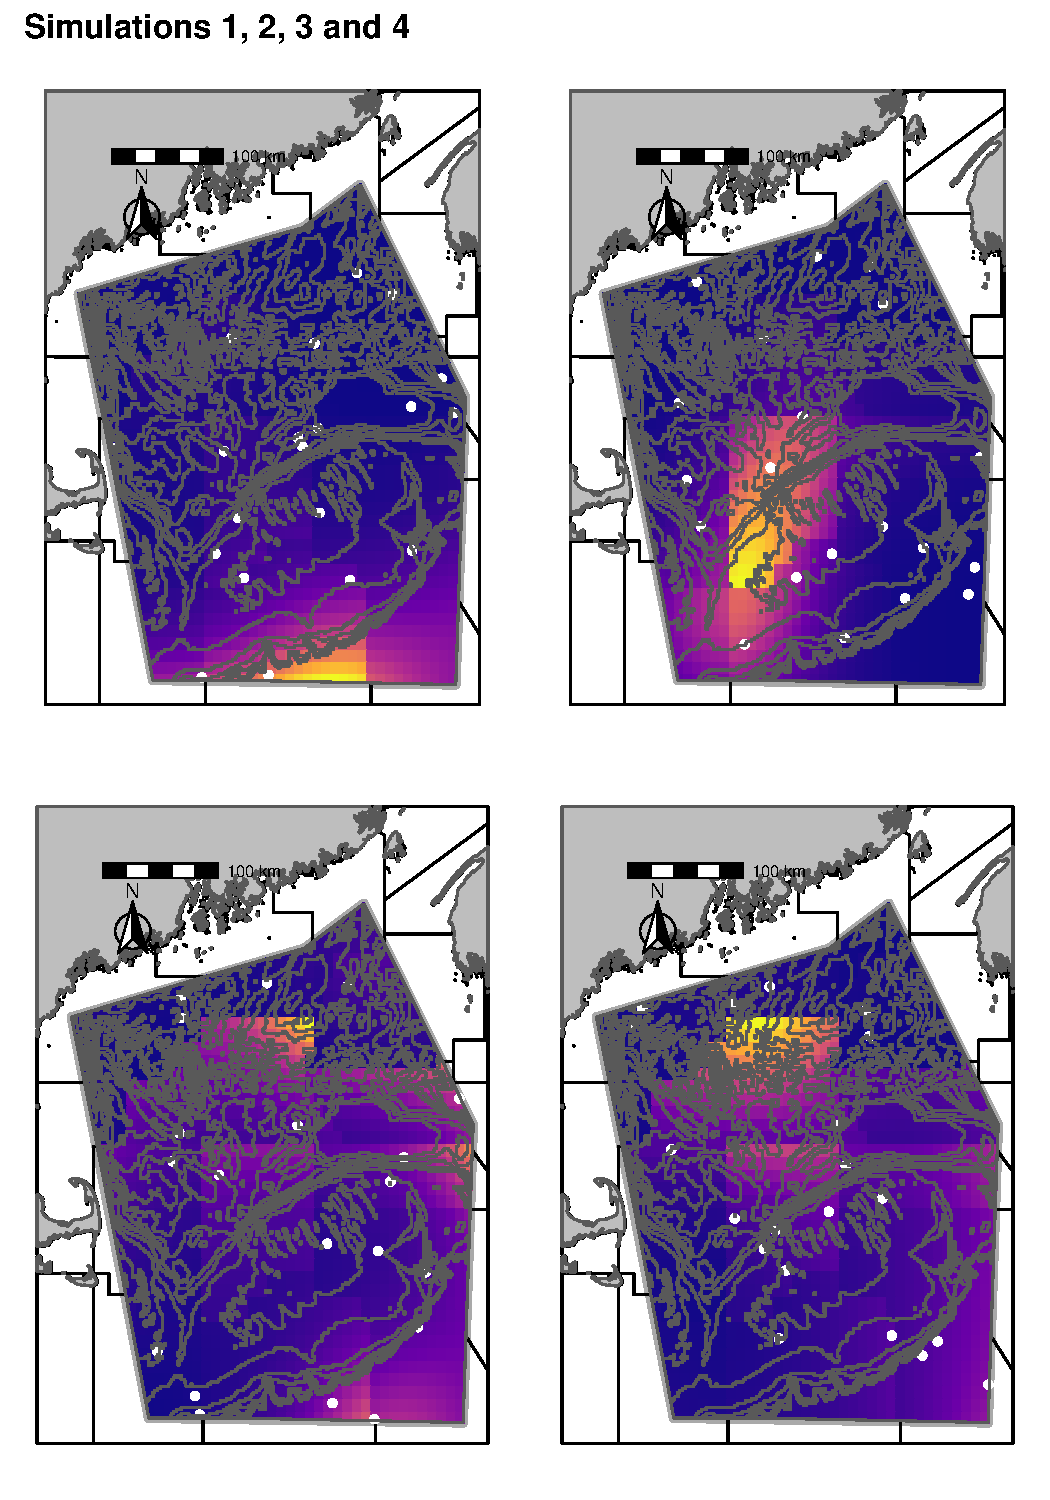
\includegraphics{Survey_tutortial_files/figure-latex/depth-samp-plt-1.pdf}
\caption{\label{fig:depth-samp-plt}Biomass distribution with the Depth survey stations overlain and the Depth stratification polygons overlain.}
\end{figure}

\hypertarget{now-we-can-compare-the-random-survey-estimates-to-the-depth-and-nafo-stratified-surveys.}{%
\section{Now we can compare the random survey estimates to the depth and NAFO stratified surveys.}\label{now-we-can-compare-the-random-survey-estimates-to-the-depth-and-nafo-stratified-surveys.}}

\begin{figure}
\centering
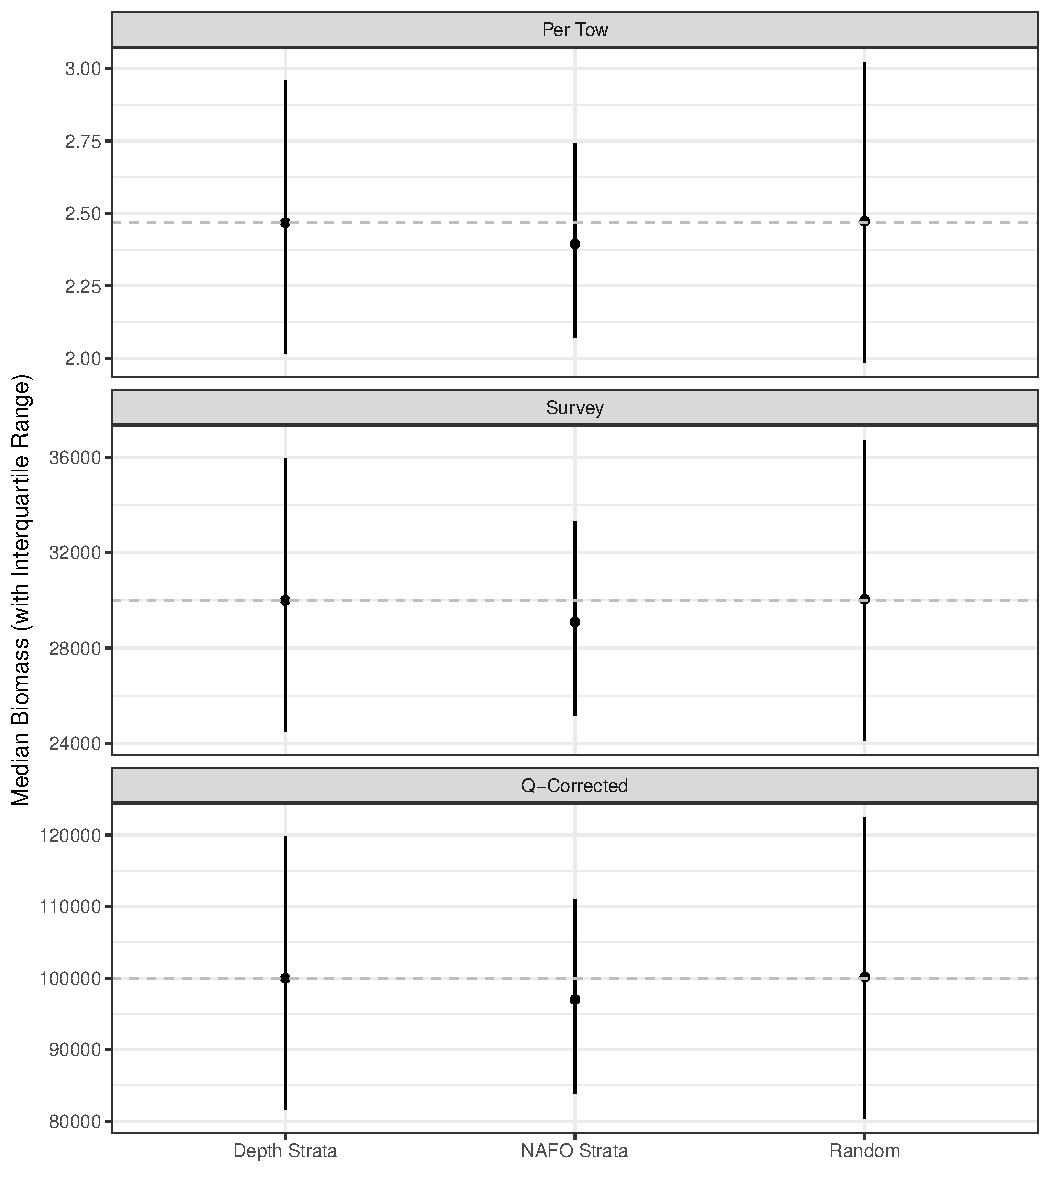
\includegraphics{Survey_tutortial_files/figure-latex/bm-plts-1.pdf}
\caption{\label{fig:bm-plts}Biomass estimates from the 3 different survey sampling schemes. When the number of simulations run = 1 this provides the mean and 95\% CI from that simulation. When the number of simulations is \textgreater1 and \textless{} 10 the mean biomass for each simulation is shown. When the number of simulations is \textgreater=10 we show the median biomass of the simulations along with the interquartile range of the biomass from the simulations}
\end{figure}

\end{document}
